\section{Discussion}
\label{sec:discussion}

\subsection{Task 1: A2C in \pendulum}
\label{sec:task1-discussion}

The A2C algorithm was implemented and tested in the \pendulum environment.
The training process involved collecting samples, computing the policy gradient, and updating the model parameters.
The results indicate that A2C is capable of learning a policy that effectively balances the pendulum, achieving a reward over -150 after training for 1000 episodes.

\subsubsection{Traning Command}
The training command used for this task was:
\begin{minted}{bash}
python a2c_pendulum.py --device cpu --exp report
\end{minted}

The hyperparameters used for training were:
\begin{itemize}
    \item \texttt{device}: \texttt{cpu}
    \item \texttt{actor-lr}: $3\times 10^{-4}$
    \item \texttt{critic-lr}: $3\times 10^{-3}$
    \item \texttt{discount-factor}: $0.9$
    \item \texttt{num-episodes}: $1000$
    \item \texttt{eval-episodes}: $5$
    \item \texttt{seed}: $42$
    \item \texttt{entropy-weight}: $0.01$
\end{itemize}

As the number of episodes are set to 1000, the model will be trained for at most 200k steps.
Since it can achieve a reward over -150 after 1000 episodes that match the full grade requirement, I stop the training process at this point.
But if you want to train the model for more episodes, you can set the \texttt{num-episodes} to a larger number.

\subsubsection{Training Curve}
The training curve for the A2C algorithm in the \pendulum environment is shown in Figure \ref{fig:task1}.
The x-axis represents the number of environment steps taken, while the y-axis shows the average reward obtained at evaluation.

\begin{figure}[H]
    \centering
    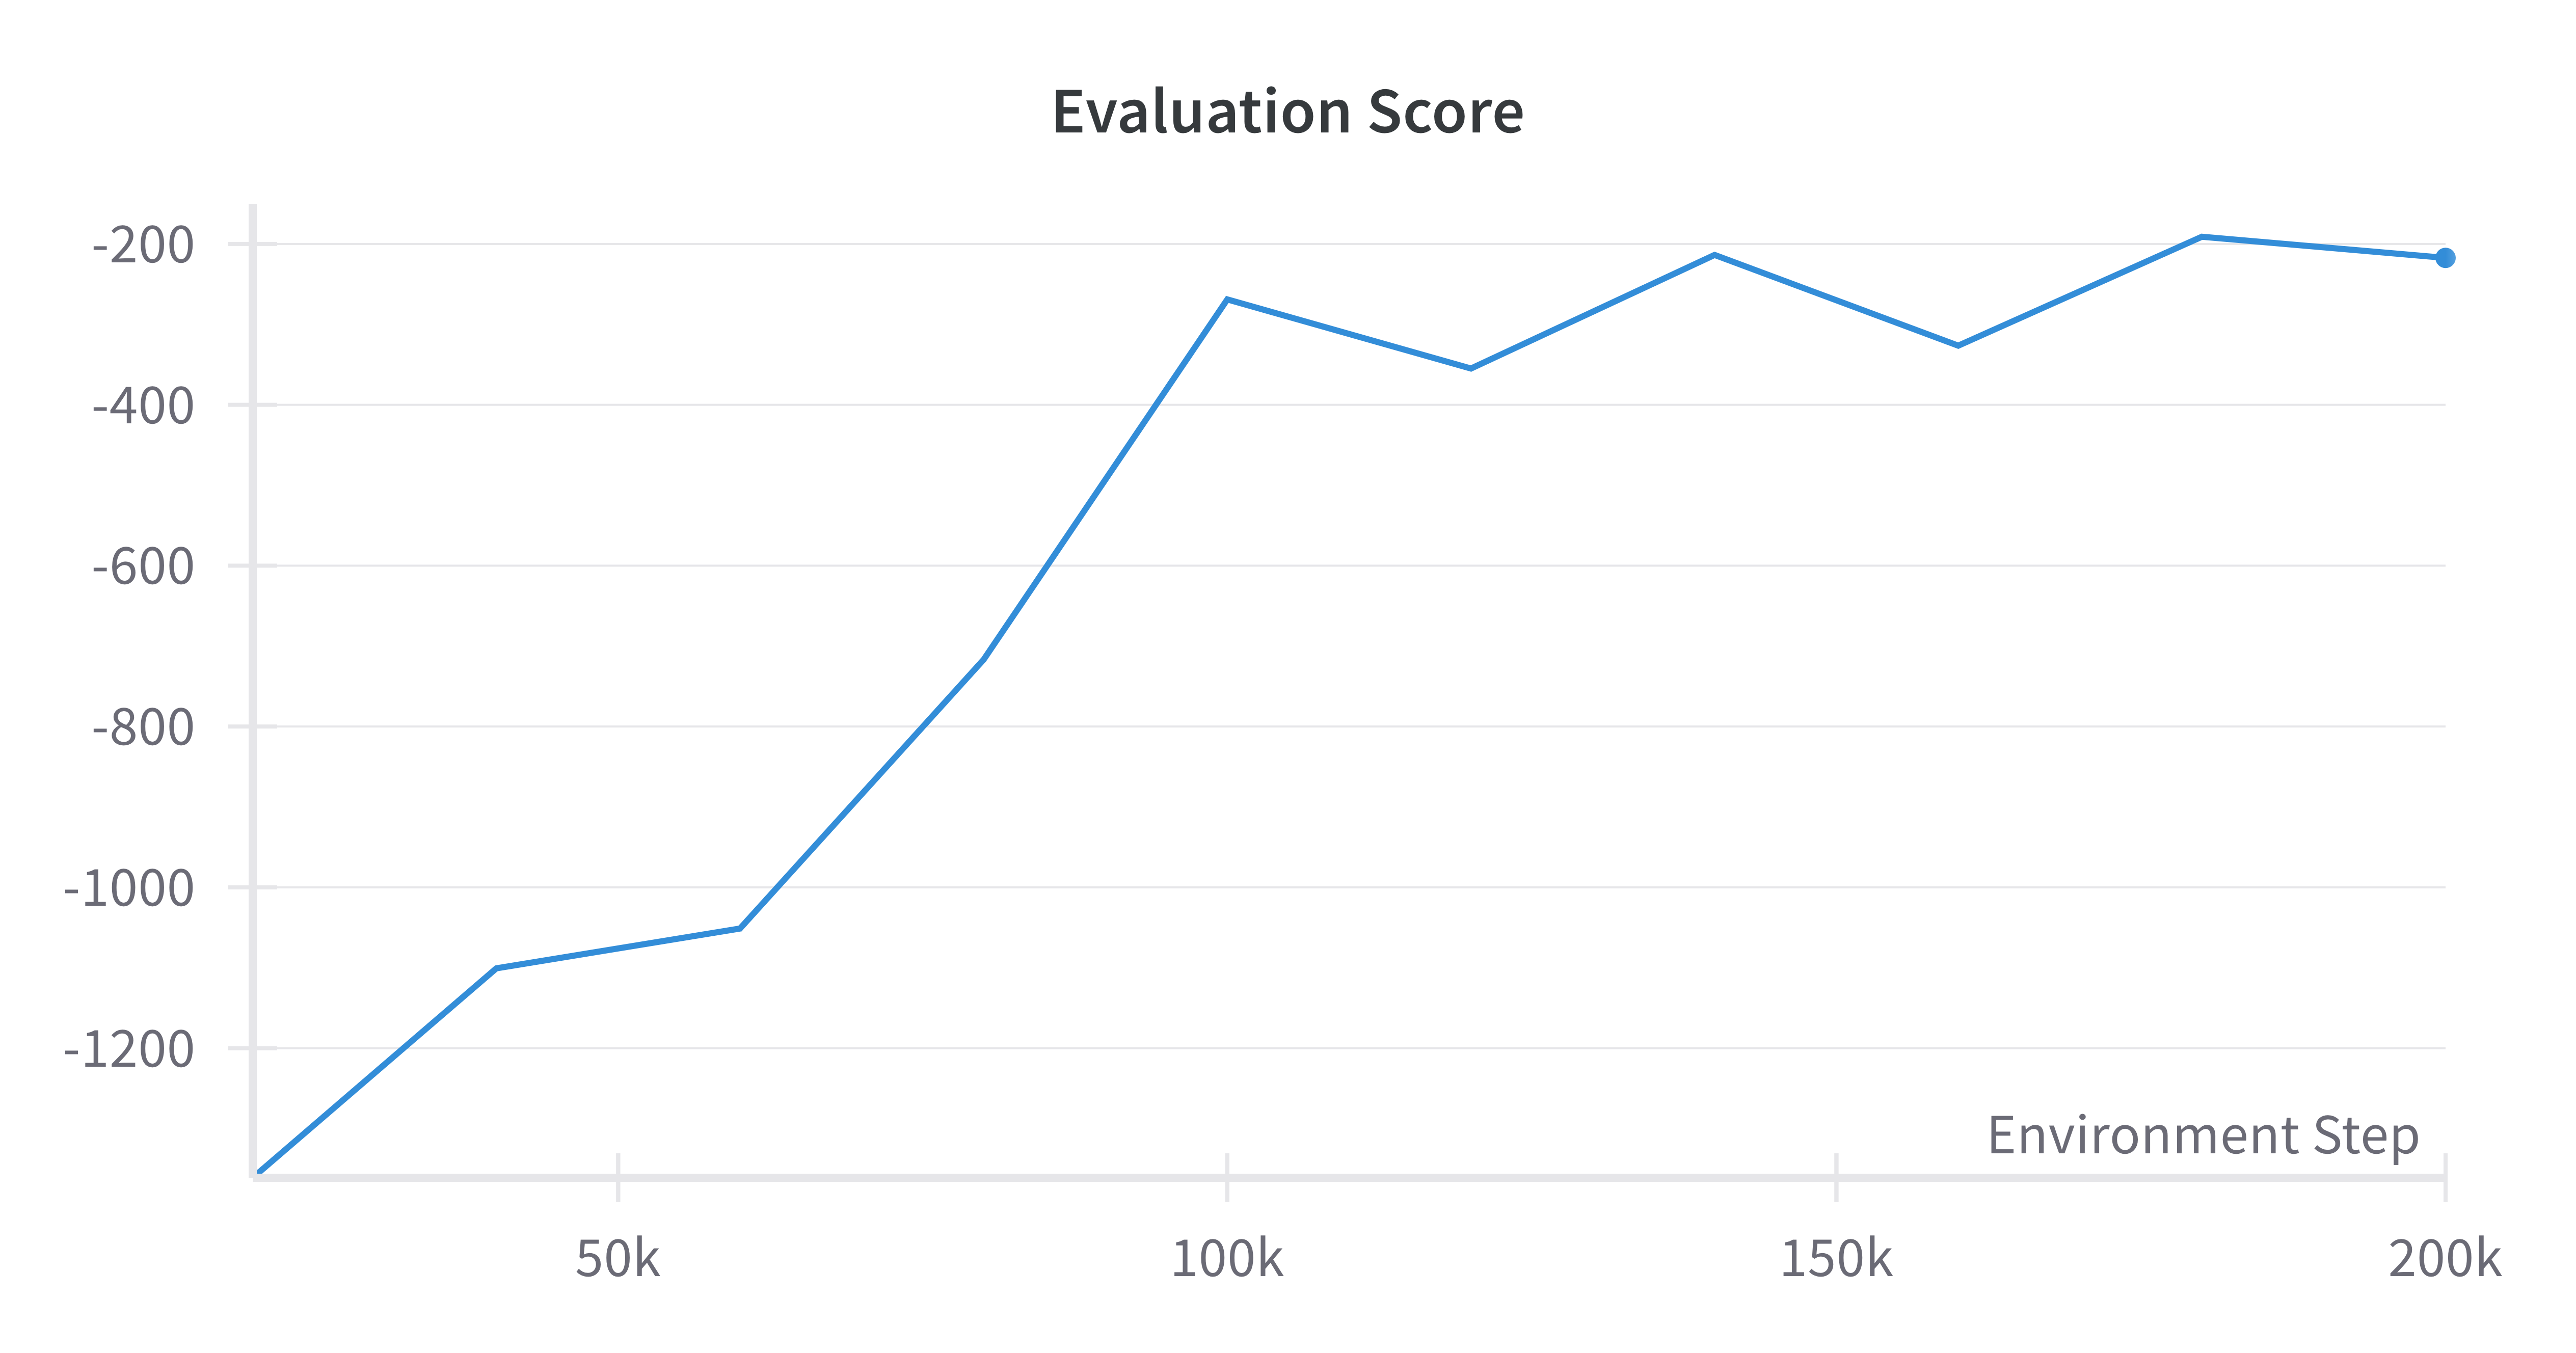
\includegraphics[width=0.8\textwidth]{figures/task1.png}
    \caption{A2C training curve in the \pendulum environment.}
    \label{fig:task1}
\end{figure}

\subsubsection{Testing Command}

\begin{minted}{bash}
python3 a2c_pendulum.py --device cpu --mode test --ckpt results/task1/report/a2c_best.pth --seed 210114487
\end{minted}

The seed set for testing is 210114487, which is just a random number to ensure the reproducibility of the results.
The testing environment's seed are not picked by any specific rule, but just generated by adding from the specified seed.
That is, the testing environment's seed is 210114487 + i, where i is the index of the testing environment.

For the first task, I can achieve reward -111.6 over 20 consecutive testing episodes using the best checkpoint trained in 200k environment steps.

\subsection{Task 2: PPO-Clip with GAE on \pendulum}
\label{sec:task2-discussion}

The PPO-Clip algorithm was implemented and tested in the \pendulum environment.
The training process involved collecting samples, computing the policy gradient, and updating the model parameters.
The results indicate that PPO-Clip is capable of learning a policy that effectively balances the pendulum, achieving a reward over -150 after training for 200k environment steps.

\subsubsection{Training Command}

The training command used for this task was:
\begin{minted}{bash}
python3 ppo_pendulum.py --device cpu --exp report
\end{minted}

The hyperparameters used for training were:
\begin{itemize}
    \item \texttt{device}: \texttt{cpu}
    \item \texttt{actor-lr}: $1\times 10^{-4}$
    \item \texttt{critic-lr}: $3\times 10^{-4}$
    \item \texttt{discount-factor}: $0.9$
    \item \texttt{num-episodes}: $100$
    \item \texttt{eval-episodes}: $5$
    \item \texttt{seed}: $42$
    \item \texttt{entropy-weight}: $0.01$
    \item \texttt{batch-size}: $128$
    \item \texttt{epsilon}: $0.2$
    \item \texttt{rollout-len}: $2000$
\end{itemize}

As the number of episodes are set to 100, the model will be trained for at most 200k steps.
Since it can achieve a reward over -150 after 1000 episodes that match the full grade requirement, I stop the training process at this point.
But if you want to train the model for more episodes, you can set the \texttt{num-episodes} to a larger number.

\subsubsection{Training Curve}

The training curve for the PPO-Clip algorithm in the \pendulum environment is shown in Figure \ref{fig:task2}.
The x-axis represents the number of environment steps taken, while the y-axis shows the average reward obtained at evaluation.
The evaluation is performed every 20k environment steps, and the average reward is calculated over 5 episodes.

\begin{figure}[H]
    \centering
    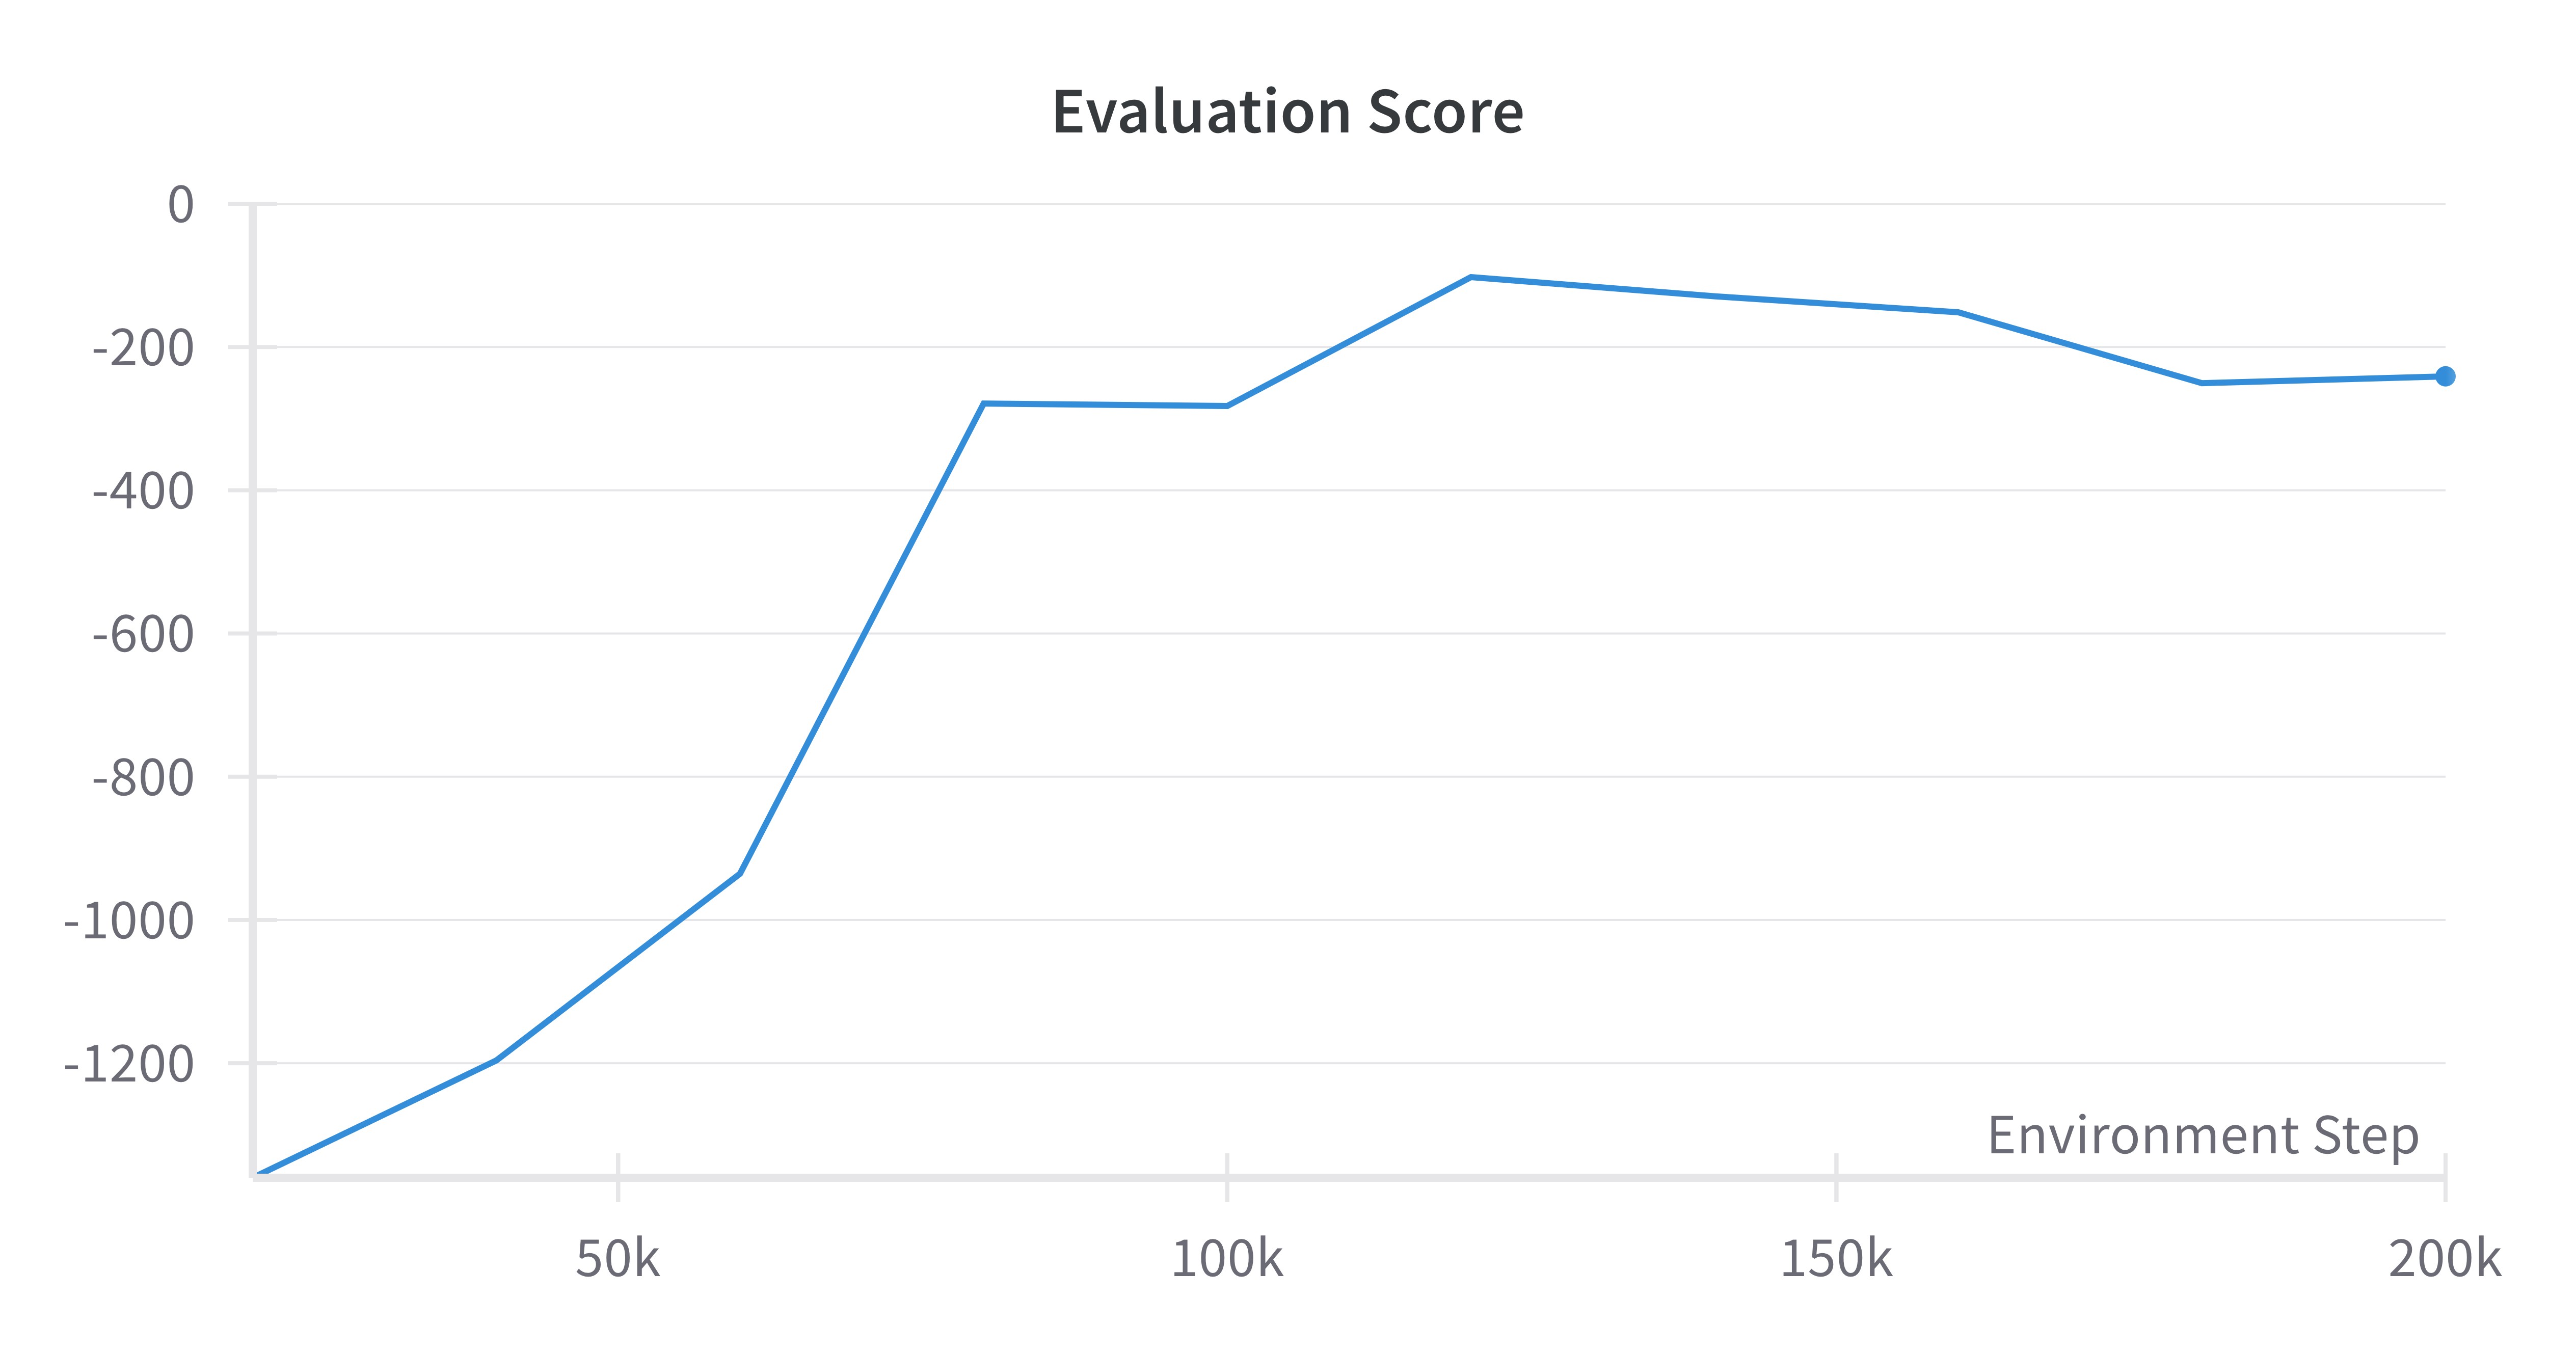
\includegraphics[width=0.8\textwidth]{figures/task2.png}
    \caption{PPO-Clip training curve in the \pendulum environment.}
    \label{fig:task2}
\end{figure}
The training curve shows that the PPO-Clip algorithm is able to learn a policy that effectively balances the pendulum, achieving a reward over -150 after training for 200k environment steps.
The training process was set to 200k environment steps, and the model was trained for at most 200k steps.

\subsubsection{Testing Command}

\begin{minted}{bash}
python3 ppo_pendulum.py --device cpu --mode test --ckpt results/task2/report/ppo_best.pth --seed 1708180417
\end{minted}

Same as above, the seed set for testing is 1708180417, which is just a random number to ensure the reproducibility of the results.
The testing environment's seed are not picked by any specific rule, but just generated by adding from the specified seed.
That is, the testing environment's seed is 1708180417 + i, where i is the index of the testing environment.

For the second task, I can achieve reward -96.90 over 20 consecutive testing episodes using the best checkpoint trained in 200k environment steps.

\subsection{Task 3: PPO-Clip with GAE on \walker}
\label{sec:task3-discussion}

The PPO algorithm was implemented and tested in the \walker environment.
The training process involved collecting samples, computing the policy gradient, and updating the model parameters.
The results indicate that PPO is capable of learning a policy that effectively balances the walker, achieving a reward over 2500 after training for 1,000,000 environment steps.

\subsubsection{Training Command}

The training command used for this task was:
\begin{minted}{bash}
python3 ppo_walker.py --device cuda --exp report
\end{minted}

The hyperparameters used for training were:
\begin{itemize}
    \item \texttt{device}: \texttt{cpu}
    \item \texttt{actor-lr}: $1\times 10^{-4}$
    \item \texttt{critic-lr}: $3\times 10^{-4}$
    \item \texttt{discount-factor}: $0.99$
    \item \texttt{num-episodes}: $400$
    \item \texttt{eval-episodes}: $5$
    \item \texttt{seed}: $42$
    \item \texttt{entropy-weight}: $0.01$
    \item \texttt{batch-size}: $64$
    \item \texttt{epsilon}: $0.2$
    \item \texttt{rollout-len}: $2500$
\end{itemize}

As the number of episodes are set to 400, and the rollout length is set to 2500, the model will be trained for at most 1,000,000 steps.
Since it can achieve a reward over 2500 after 1,000,000 steps that match the full grade requirement, I stop the training process at this point.
But if you want to train the model for more episodes, you can set the \texttt{num-episodes} or \texttt{rollout-len} to a larger number.

\subsubsection{Training Curve}

The training curve for the PPO-Clip algorithm in the \walker environment is shown in Figure \ref{fig:task3}.
The x-axis represents the number of environment steps taken, while the y-axis shows the average reward obtained at evaluation.
The evaluation is performed every 25 episodes, and the average reward is calculated over 5 episodes.

\begin{figure}[H]
    \centering
    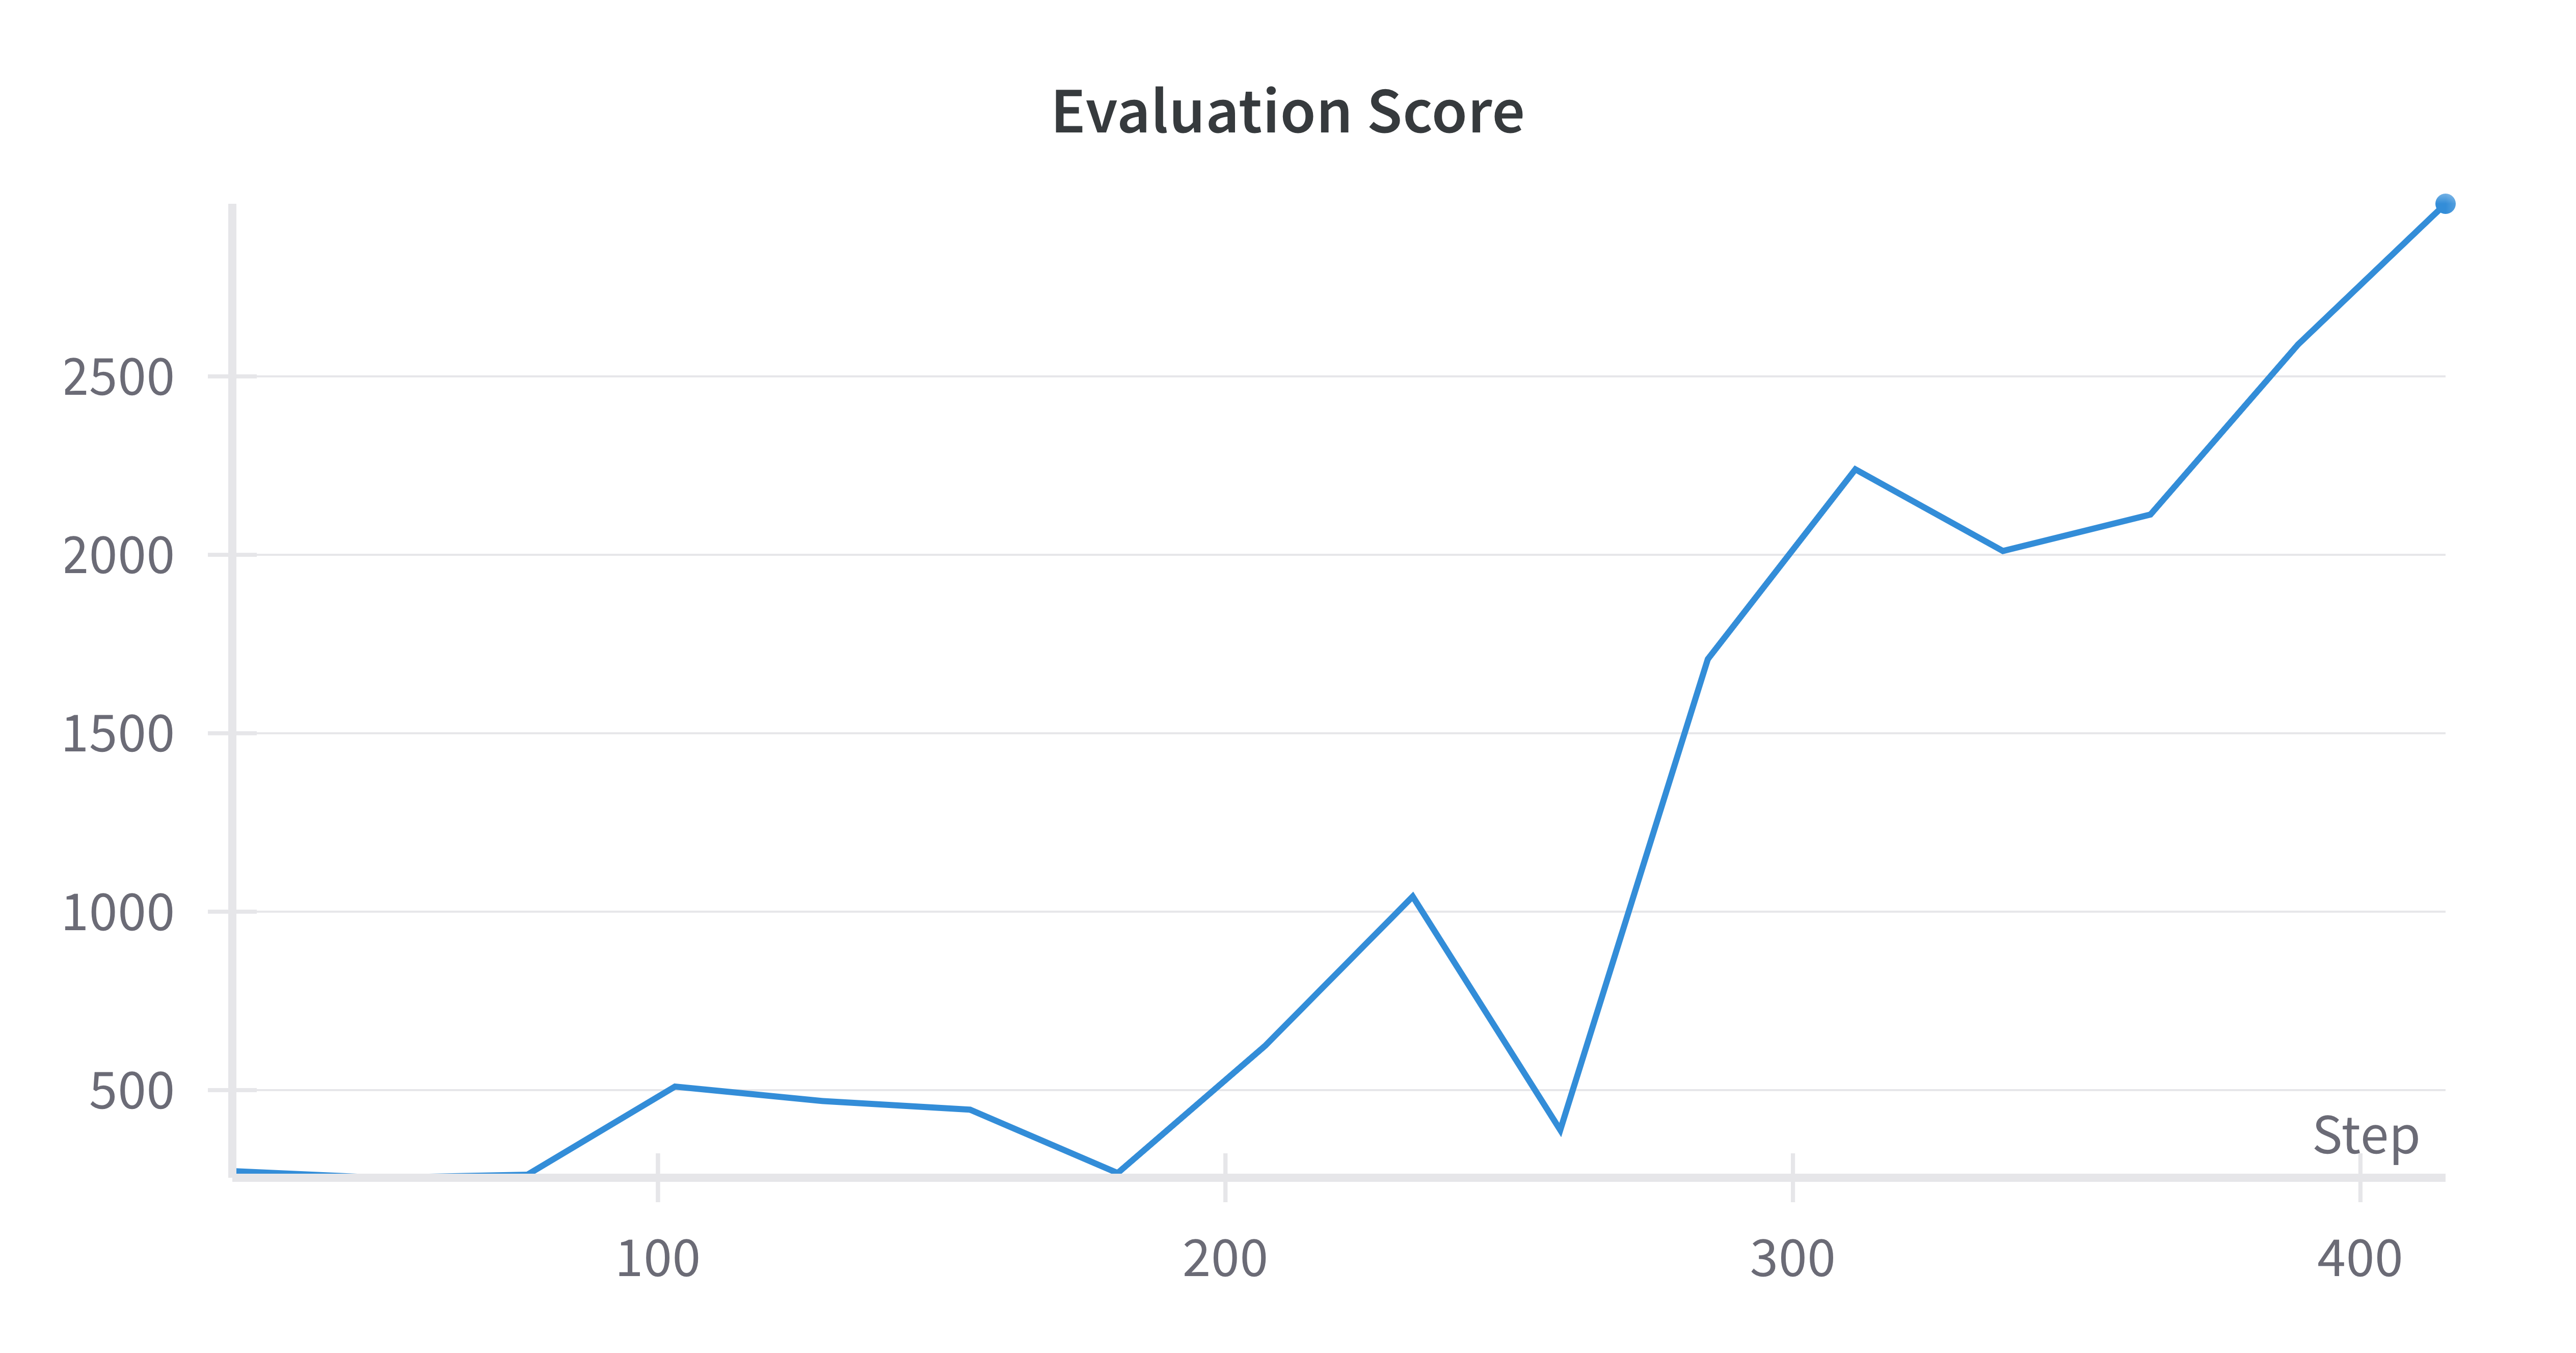
\includegraphics[width=0.8\textwidth]{figures/task3.png}
    \caption{PPO-Clip training curve in the \walker environment.}
    \label{fig:task3}
\end{figure}
The training curve shows that the PPO-Clip algorithm is able to learn a policy that effectively balances the walker, achieving a reward over 2500 after training for 1,000,000 environment steps.
The training process was set to 400 episodes, and the model was trained for at most 1,000,000 steps.

\subsubsection{Testing Command}

\begin{minted}{bash}
python3 ppo_walker.py --device cpu --mode test --ckpt results/task3/report/ppo_best.pth --seed 2139949224
\end{minted}

Same as above, the seed set for testing is 2139949224, which is just a random number to ensure the reproducibility of the results.
If you want to test the model in a different environment, you can set the \texttt{seed} to a different number.
It is possible to lead to different results, but the model should still be able to achieve a reward over 3,500 for a very high probability.
The testing environment's seed are not picked by any specific rule, but just generated by adding from the specified seed.
That is, the testing environment's seed is 2139949224 + i, where i is the index of the testing environment.

For the third task, I can achieve reward 3655.76 over 20 consecutive testing episodes using the best checkpoint trained in 1,000,000 environment steps.
